\documentclass[pdftex,english,oribibl]{llncs}

%%%%%%%%%%%%%%%%%%%%%%%%%%%%%%%%%%%%%%%%%%%%%%%%%%%%%%%%%%%%%%%%%%%%%%%%%%%%%%%%%%%%%%%%%%%%
%%% Spracheinstellungen laden
%%%%%%%%%%%%%%%%%%%%%%%%%%%%%%%%%%%%%%%%%%%%%%%%%%%%%%%%%%%%%%%%%%%%%%%%%%%%%%%%%%%%%%%%%%%%
\usepackage[english]{babel}

%%%%%%%%%%%%%%%%%%%%%%%%%%%%%%%%%%%%%%%%%%%%%%%%%%%%%%%%%%%%%%%%%%%%%%%%%%%%%%%%%%%%%%%%%%%%
%%% Schriftart in der Ausgabe/Eingabe
%%%%%%%%%%%%%%%%%%%%%%%%%%%%%%%%%%%%%%%%%%%%%%%%%%%%%%%%%%%%%%%%%%%%%%%%%%%%%%%%%%%%%%%%%%%%
\usepackage[T1]{fontenc}
\usepackage{textcomp}
\usepackage[latin1]{inputenc}

%%%%%%%%%%%%%%%%%%%%%%%%%%%%%%%%%%%%%%%%%%%%%%%%%%%%%%%%%%%%%%%%%%%%%%%%%%%%%%%%%%%%%%%%%%%%
%%% Farben
%%%%%%%%%%%%%%%%%%%%%%%%%%%%%%%%%%%%%%%%%%%%%%%%%%%%%%%%%%%%%%%%%%%%%%%%%%%%%%%%%%%%%%%%%%%%
\usepackage{xcolor}

%%%%%%%%%%%%%%%%%%%%%%%%%%%%%%%%%%%%%%%%%%%%%%%%%%%%%%%%%%%%%%%%%%%%%%%%%%%%%%%%%%%%%%%%%%%%
%%% Zitate
%%%%%%%%%%%%%%%%%%%%%%%%%%%%%%%%%%%%%%%%%%%%%%%%%%%%%%%%%%%%%%%%%%%%%%%%%%%%%%%%%%%%%%%%%%%%
\usepackage[numbers]{natbib}
\bibliographystyle{abbrvnat}
%\bibliographystyle{dinat}
%\bibliographystyle{plainnat}
%\bibliographystyle{splncs}
%% Similar to option "sectionbib" but \refname instead of \bibname
\makeatletter
\renewcommand\bibsection{\section*{\refname\@mkboth{\MakeUppercase{\refname}}{\MakeUppercase{\refname}}}}
\makeatother

%%%%%%%%%%%%%%%%%%%%%%%%%%%%%%%%%%%%%%%%%%%%%%%%%%%%%%%%%%%%%%%%%%%%%%%%%%%%%%%%%%%%%%%%%%%%
%%% Index
%%%%%%%%%%%%%%%%%%%%%%%%%%%%%%%%%%%%%%%%%%%%%%%%%%%%%%%%%%%%%%%%%%%%%%%%%%%%%%%%%%%%%%%%%%%%
%\usepackage{makeidx}
%\makeindex

%% PDF Einstellungen
% muss nach natbib geladen werden!
\usepackage{nameref}
\usepackage{varioref}
\usepackage[pdfusetitle,pdftex,colorlinks]{hyperref}
\hypersetup{pdfborder={0 0 0}}
\hypersetup{bookmarksdepth=3}
\hypersetup{bookmarksopen=true}
\hypersetup{bookmarksopenlevel=1}
\hypersetup{bookmarksnumbered=true}
\usepackage{color}
\hypersetup{colorlinks=false}

%\usepackage[section]{tocbibind}

\makeatletter
\gdef\@keywords{}
\def\keywords#1{\gdef\@keywords{#1}}
\gdef\@subtitle{}
\def\subtitle#1{\gdef\@subtitle{#1}}

%% modified from llncs
\renewenvironment{abstract}{%
  \list{}{\advance\topsep by0.35cm\relax\small%
          \leftmargin=1cm%
          \labelwidth=\z@%
          \listparindent=\z@%
          \itemindent\listparindent%
          \rightmargin\leftmargin}%
          \item[\hskip\labelsep\bfseries\abstractname]}{%
  \if!\@keywords!\else{\item[~]\item[\hskip\labelsep\bfseries\keywordname]\@keywords}\fi%
  \endlist}

\AtBeginDocument{%
  \if!\@subtitle!\else\hypersetup{pdfsubject={\@subtitle}}\fi
  \if!\@keywords!\else\hypersetup{pdfkeywords={\@keywords}}\fi
}
\makeatother

% llncs hyperref fix
\makeatletter
\providecommand*{\toclevel@author}{0}
\providecommand*{\toclevel@title}{0}
\makeatother

%%%%%%%%%%%%%%%%%%%%%%%%%%%%%%%%%%%%%%%%%%%%%%%%%%%%%%%%%%%%%%%%%%%%%%%%%%%%%%%%%%%%%%%%%%%%
%%% Grafiken
%%%%%%%%%%%%%%%%%%%%%%%%%%%%%%%%%%%%%%%%%%%%%%%%%%%%%%%%%%%%%%%%%%%%%%%%%%%%%%%%%%%%%%%%%%%%
\usepackage[pdftex]{graphicx}
\DeclareGraphicsExtensions{.pdf,.jpg,.png}
\usepackage{subfigure}

%%%%%%%%%%%%%%%%%%%%%%%%%%%%%%%%%%%%%%%%%%%%%%%%%%%%%%%%%%%%%%%%%%%%%%%%%%%%%%%%%%%%%%%%%%%%
%%% Mathe
%%%%%%%%%%%%%%%%%%%%%%%%%%%%%%%%%%%%%%%%%%%%%%%%%%%%%%%%%%%%%%%%%%%%%%%%%%%%%%%%%%%%%%%%%%%%
\usepackage{amsmath}
\usepackage{amssymb}

%%%%%%%%%%%%%%%%%%%%%%%%%%%%%%%%%%%%%%%%%%%%%%%%%%%%%%%%%%%%%%%%%%%%%%%%%%%%%%%%%%%%%%%%%%%%
%%% Listings
%%%%%%%%%%%%%%%%%%%%%%%%%%%%%%%%%%%%%%%%%%%%%%%%%%%%%%%%%%%%%%%%%%%%%%%%%%%%%%%%%%%%%%%%%%%%
\usepackage{listings}
%\lstset{escapechar=\%, frame=tb, basicstyle=\footnotesize}

%\definecolor{colorOperator}{HTML}{0.05,0.7,0.05}
%\definecolor{colorComment}{HTML}{0.8,0.5,0}
%\definecolor{colorKeyword}{HTML}{0,0.2,1.0}
%\definecolor{colorConsole}{HTML}{0.5,0,0.8}

\definecolor{black}{HTML}{000000}
\definecolor{red}{HTML}{FF0000}
\definecolor{green}{HTML}{00FF00}
\definecolor{blue}{HTML}{0000FF}
\definecolor{white}{HTML}{FFFFFF}
\definecolor{lightgray}{HTML}{EEEEEE}

\definecolor{colorOperator}{HTML}{007700}
\definecolor{colorNumber}{HTML}{FF77FF}
\definecolor{colorComment}{HTML}{777700}
\definecolor{colorKeyword}{HTML}{000000}
\definecolor{colorConsole}{HTML}{000000}
\definecolor{colorString}{HTML}{AAAA00}

\lstdefinestyle{Java}{
	backgroundcolor=\color{white},
	basicstyle=\footnotesize,
	keywordstyle=\color{colorKeyword},
	stringstyle=\color{colorString},
	commentstyle=\color{colorComment},
	rulecolor=\color{black},
	numberstyle=\scriptsize,
	breakatwhitespace=false,
	breaklines=true,
	captionpos=b,
	deletekeywords={...},
	escapeinside={\%*}{*)},
	extendedchars=true,
	gobble=4,
	keepspaces=true,
	language=Java,
	morekeywords={null,...},
	numbers=left,
	stepnumber=1,
	numbersep=8pt,
	breaklines=true,
	frame=single,
	showspaces=false,
	showstringspaces=false,
	showtabs=false,
	stepnumber=1,	
	tabsize=4,
	literate=
		{0}{{{\color{colorNumber}0}}}{1}
		{1}{{{\color{colorNumber}1}}}{1}
		{2}{{{\color{colorNumber}2}}}{1}
		{3}{{{\color{colorNumber}3}}}{1}
		{4}{{{\color{colorNumber}4}}}{1}
		{5}{{{\color{colorNumber}5}}}{1}
		{6}{{{\color{colorNumber}6}}}{1}
		{7}{{{\color{colorNumber}7}}}{1}
		{8}{{{\color{colorNumber}8}}}{1}
		{9}{{{\color{colorNumber}9}}}{1}
		{=}{{{\color{colorOperator}=}}}1
		{!}{{{\color{colorOperator}!}}}1
		{\&}{{{\color{colorOperator}\&}}}1
		{*}{{{\color{colorOperator}*}}}1
		{.}{{{\color{colorOperator}.}}}1
		{,}{{{\color{colorOperator},}}}1
		{:}{{{\color{colorOperator}:}}}1
		{;}{{{\color{colorOperator};}}}1
		{(}{{{\color{colorOperator}(}}}1
		{)}{{{\color{colorOperator})}}}1
		{<}{{{\color{colorOperator}$<$}}}1
		{>}{{{\color{colorOperator}$>$}}}1
		{[}{{{\color{colorOperator}[}}}1
		{]}{{{\color{colorOperator}]}}}1
		{\{}{{{\color{colorOperator}\{}}}1
		{\}}{{{\color{colorOperator}\}}}}1
}

\lstdefinestyle{JSON}{
	basicstyle=\normalfont\ttfamily,
	numbers=left,
	numberstyle=\footnotesize,
	stringstyle=\color{colorString},
	backgroundcolor=\color{lightgray},
	stepnumber=1,
	numbersep=8pt,
	showstringspaces=false,
	extendedchars=true,
	breaklines=true,
	keepspaces=true,
	showspaces=false,
	showstringspaces=false,
	showtabs=false,
	frame=single,
	showspaces=false,
	showstringspaces=false,
	showtabs=false,
	stepnumber=1,	
	tabsize=4,
	literate=
		{0}{{{\color{colorNumber}0}}}{1}
		{1}{{{\color{colorNumber}1}}}{1}
		{2}{{{\color{colorNumber}2}}}{1}
		{3}{{{\color{colorNumber}3}}}{1}
		{4}{{{\color{colorNumber}4}}}{1}
		{5}{{{\color{colorNumber}5}}}{1}
		{6}{{{\color{colorNumber}6}}}{1}
		{7}{{{\color{colorNumber}7}}}{1}
		{8}{{{\color{colorNumber}8}}}{1}
		{9}{{{\color{colorNumber}9}}}{1}
		{:}{{{\color{colorOperator}{:}}}}{1}
		{,}{{{\color{colorOperator}{,}}}}{1}
		{\{}{{{\color{colorOperator}{\{}}}}{1}
		{\}}{{{\color{colorOperator}{\}}}}}{1}
		{[}{{{\color{colorOperator}{[}}}}{1}
		{]}{{{\color{colorOperator}{]}}}}{1}
		{\{}{{{\color{colorOperator}\{}}}{1}
		{\}}{{{\color{colorOperator}\}}}}{1},
}


\lstdefinestyle{Bash}{
	backgroundcolor=\color{white},
	basicstyle=\footnotesize,
	breakatwhitespace=false,
	breaklines=true,
	breakindent=0pt,
	captionpos=b,
	commentstyle=\color{colorComment},
	deletekeywords={...},
	escapeinside={\%*}{*)},
	extendedchars=true,
	frame=single,
	keepspaces=true,
	keywordstyle=\color{colorKeyword},
	language=Bash,
	morekeywords={NULL, nullptr,...},
	rulecolor=\color{black},
	showspaces=false,
	showstringspaces=false,
	showtabs=false,
	stepnumber=1,
	stringstyle=\color{colorString},
	tabsize=4,
	literate=	{\$}{{{\color{colorConsole}\$}}}1
}

%%% Sonstiges
%%%%%%%%%%%%%%%%%%%%%%%%%%%%%%%%%%%%%%%%%%%%%%%%%%%%%%%%%%%%%%%%%%%%%%%%%%%%%%%%%%%%%%%%%%%%
\newcommand{\TODO}[1]{\par\textcolor{red}{#1}\marginpar{\textcolor{red}{TODO}}}
\newcommand{\TODOX}[1]{\textcolor{red}{#1}\marginpar{\textcolor{red}{TODO}}}
\pagestyle{plain}

% Keine "Schusterjungen"
\clubpenalty = 10000
% Keine "Hurenkinder"
\widowpenalty = 10000 \displaywidowpenalty = 10000


%%%%%%%%%%%%%%%%%%%%%%%%%%%%%%%%%%%%%%%%%%%%%%%%%%%%%%%%%%%%%%%%%%%%%%%%%%%%%%%
%%% BEGIN DOCUMENT
%%%%%%%%%%%%%%%%%%%%%%%%%%%%%%%%%%%%%%%%%%%%%%%%%%%%%%%%%%%%%%%%%%%%%%%%%%%%%%%
\title{Simulation-based Resilience Prediction of Microservice Architectures}
% \subtitle{My (optional) Subtitle}
\author{Samuel Beck, Johannes G�nth�r, Christoph Zorn}
\institute{University of Stuttgart\\Reliable Software Systems (RSS)\\70569 Stuttgart, Germany}


\begin{document}

\maketitle

\begin{abstract}
	Current software simulators are tailored towards one specific purpose of conservative software simulation. Given the success of these tools it would be useful to run these tools on microservice architectures. This paper will focus on the development of a simulator that can be used for microservice architectures.
\end{abstract}

\section{Introduction}\label{sec:introduction}

	Was rein muss: Was wir wollen (unser ziel), ...
	in section 2 steht : the problem we are currently facing. Dieses problem muss hier oder vor section 2 erkl�rt werden  
	
	%This is my introduction. %\citet{Shaw2003WritingGoodSoftwareEngineeringResearchPapersMinitutorial} wrote a paper with %hints on how to write good software engineering research papers. By the way, this was an %example for using the \textit{natbib} command \texttt{\textbackslash{}citet\{\}}.
	
	%Section~\ref{sec:anotherSection} presents everything one must know. The conclusions follow %in Section~\ref{sec:conclusions}.

%\section{Another Section}\label{sec:anotherSection}
	
	%\textit{AspectJ} can be used to weave cross-cutting concerns into Java programs %\citep{AspectJ2007}. By the way, this was an example for using the \textit{natbib} command %\texttt{\textbackslash{}citep\{\}}.
	
	%We will now demonstrate how to use subfigures (see Figure~\ref{fig:subfig}). %Figure~\ref{fig:circle} shows a circle. A star is displayed in Figure~\ref{fig:star}.
	
	%\begin{figure}
		% \centering
		%\subfigure[This is a circle.]{\label{fig:circle}
		 % 
\includegraphics[width=0.3\textwidth]{figures/template_circle.pdf}
		%}
		%\subfigure[This is a star.]{\label{fig:star}
		%  
\includegraphics[width=0.3\textwidth]{figures/template_star.pdf}
		%}
		%\caption{A circle (a) and a star (b). Note that any caption ends with a full stop %character.}
		% \label{fig:subfig}
	%\end{figure}
  
\section{Research}\label{sec:research}

	Before developing a new tool we looked around to see what software solutions are currently available to simulate a MS architecture. To get a sense of the functionality of the tools, we analyzed multiple different simulators in depth to see if their functionality would solve the problem we are currently facing. This section gives a brief overview of the functionalities of the four simulators and the pros and cons on why to use them as an codebase for our future tool.

\subsection{Tool Evaluation with Regard to Sutability for the Adaptation for Microservice Arcitectures}\label{subsec:toolsInComparison}

\subsubsection{Spigo}
	
	During our research on existing tools for microservice simulation we discovered a tool called spigo. It was written by Adrian Cockcroft a Amazon Web Services employee in the programming language go. Therefore the name spigo comes from Simulate Protocol Interactions in Go. \newline On the first view the tool looked very promising. Spigo contains a fairly simple JSON input and the structure of the parameters is intuitive. Each microservice architecture consists of multiple microservices. Each microservice has a name, a package inheritance a counter of the instances and dependencies to other microservices. The reason we like this tool is because it can simulate the occurrence of an error. Spigo uses the error monkeys from the simian army. But here lies already on of the biggest disadvantages. One can only simulate the failure of a single microservice during the execution. Another point against spigo is the weak documentation of the actual implementation as well as minor bugs that remain from 12 months ago. \newline In conclusion it is quite sure that spigo is not an option for us to use for an extension module. The restrictive and static code design makes it hard to follow the workflow and append another module.

\subsubsection{Palladio}

	Palladio is a software component model for business information systems to enable model-driven predictions on throughput, response time and resource utilization. \cite{Palladio2007} Our motivation to get familiar with Palladio was primarily initiated by Simulizar. A tool extended from Palladio which will be described later in this article. Component models provide many advantages over object-oriented development approaches i.e. higher usability, quality and better test potential. \cite{Palladio2007} This is one of the core strengths of Palladio and therefore a fact that makes it impossible for us to use it for microservices. Microservices are typically fine-grained and divided systems which means that a service knows hardly anything or nothing about the other services. A component based solution would lead our aim into the opposite direction. Every microservice would instantiated as a separate component and as a result the whole architecture would blow up in size.

\subsubsection{Simulizar}
	
	Simulizar is an extension of Palladio. This tool was especially developed for systems that change at runtime i.e. cloudcomputing and virtualized infrastructure environments. Such dynamic system adapt to the environment in order to meet the quality-of-service requirements. In the most cases software systems rely on static and fixed resource management so only steady states can be predicted.\cite{Simulizar2013} Simulizar uses the so called MAPE-K feedback loop (Monitor, Analyze, Plan, Execute, Knowledge) which is used to react to changes that are done during runtime. \newline During our research we came across a presentation on Palladio. One of the developer explained us how the project is built up and what dependent modules are needed to run a simulation. It was also mentioned that other attempts to generate an extension resulted in code duplications of functions that were already implemented but where not detected because of the huge code base. \newline
	Palladio and especially Simulizer seem to be to complex and big to get an understanding of the tool in depth. The sheer amount of code and resources that is used for collecting data and making prediction would be just an overhead on the problems that we currently face.
	

\subsubsection{GreenCloud} 

	With this tool we tried a different approach. Greencloud was designed to calculate the energy consumption of datacenters\citep[P.1]{GreenCloud}. Knowing that this was kind of a long shot we had the idea to take a simulator that simulates distributed objects and map microservice abilities and requirements to these objects. Since the simulator was written to overlook datacenters and their components, a mapping would mean that the entire microservice system would be mapped to a datacenter in the current GreenCloud simulator. Instances of microservices would compare to a server\citep[P.2]{GreenCloud} that gathers metrics. These metrics are currently power consumption, CPU- utilization and workload \citep[P.3]{GreenCloud} and should be changed or replaced to throughput,workload and whatever metrics we require from a microservice. GreenCloud also includes connections\citep[P.3]{GreenCloud} between servers. The connection could possibly used to be a mapping of microservice connections, that we can interfere to implement chaos monkeys. \newline
	Sounding good in theory but taking a closer look at the tool some problems lead to a problems. The focus of GreenCloud is obviously the simulation of power consumption. The previous mentioned connection between servers is not actually modeled but just taken into consideration regarding the power consumption of switches that connect servers together. Additionally there is no sign of the possibility to scale Instances (servers) which is a major part in a microservice system. Lastly workloads are only specified as the computing power they require (e.g. 3 Million Instructions per Second)\citep[P.3]{GreenCloud}. Communication or a differentiation between machines(DB, Workstation, ...) takes additional resources and is currently not taken into account. This would make mapping to a microservice architecture incredibly hard.  
	In hindsight it seems to be not very likely that using GreenCloud would be a good idea. The differences between provided capabilities by GreenCloud and required capabilities by the new tool is just to large. 
	
\subsubsection{CloudSim}

	Developed by the CLOUDS Laboratory of the University of Melbourne, CloudSim is a framework for modeling and simulation of cloud computing infrastructures and services. It allows modeling and simulation of large scale cloud computing data centers as well as modeling and simulation of application containers and virtualized server hosts.\cite{website_cloudsim} The platform is written in Java and extensible, in fact various extensions for the framework exist. Its architecture consists of multiple layers. The fundamental layer provides management of applications, hosts of virtual machines, etc. while the top layer represents the basic entities for hosts and enables the generation of requests in a variation of approaches, configurations and cloud scenarios.\cite{byrne2017review}
	
\section{Simulatorspecification}\label{sec:specifictation}
Like every normal software product we also wrote a specification on how the finished product should look like. The specification helped the team to get some common ground on the project and clarify what should and what should not be done. Research also helped with the specification.
We used the knowledge of simulators that we saw previously and took what we liked and included this into our own tool (e.g. Spigo input)\citep{Spigo}. 


\subsection{Input properties}\label{input}
	We want our Simulator to execute the following tasks. In order to simulate a system we need to know how the actual system is build. Therefore we will get information form an input file. This file will contain information about the infrastructure of the system. Each microservice(MS) that is part of the system has the following properties. It has a unique name, the number of instances that are used in the simulation, dependencies on other MS's, throughput and anti-patterns that it implements. See subsection \ref{subsec:reliability}.\newline
	During runtime we want to be able to modify the system by deleting some instances of microservices. We will achieve this by implementing a chaosmonkey which is inspired by netflix�s toolbox of cloud tools. There can be any number of chaosmonkey�s that need the following parameters to intercept the system. It has a Ms as a target, the number of instances it will delete and the time period in which the error will occur. Finally the input has a number of message objects that travel through the system. We expect the input to look like Figure \ref{fig:output}. A visual representation of the coded input is shown in Figure \ref{fig:SystemVisualization}  
	
\begin{figure}
\begin{lstlisting}[style=JSON]
"microservices" : {
	"Frontend": {
		"name" : "frontend",
		"antipatterns" : ["Circuit Breaker"],
		"instances": 4,
		"dependencies": ["Database", "Server"],	
		"throughput" : 3
	},
	"Database": {
		"name" : "database",
		"instances": 2,
		"dependencies": ["Frontend"],
		"throughput" : 3
	},
	"Server": {
		"name" : "server",
		"instances": 1,
		"dependencies": ["Frontend"],
		"throughput" : 3
	}
},
"message_object" : {
	"token" : {
		"instances" : 4
		"path" : ["frontend" : 5, "database" : 3]
	}
	"token: {
		"server" : 5
	}
},
"failures":	{
	"chaosmonkey" :	{
		"service" : "frontend",
		"instances" : 3,
		"time" : [1, 2, 3]	
	}
},
"triggers" : {

}\end{lstlisting}
	\caption{Input structure: The above JSON file serves for the desired input structure which represents the microservice architecture in the simulation.}
	\label{fig:output}
\end{figure}
	
	\newpage
  				
\subsection{Expected system runtime behavior}
	The basic idea of our system is that is runs on a clock. For each time period every MS will be able to send, receive and work on message objects. If a number of MS instances will go down it is expected to have larger message queues in front of a MS. As a result the system will probably slow down. To guarantee fail-safety the user will have the option to include anti-patterns in the input file. This will make a MS resilient against high workloads and failures of dependent MS. During simulation time we already gather information about performance in each timeframe to generate metrics. We also collect system failures in form of lost message objects if certain MS aren?t available anymore.
 
\subsection{Expected output metrics}
	We collect the following metrics for all MS�s. The workload, queue utilisation (size) and potential system failures due to missing instances of services. As a result there should be highlighting of eventual problematic data and an analyzation of bottlenecks and performance problems. This information will then be written into a user-friendly output file to deliver a big picture of the system.

\subsection{Supported failiure modes}
	We expect our tool to be able to disable any number of MS instances to simulate the failure of instances in the production system. The user has to define which microservices should be affected and how many instances are killed at a specific clock time. This was also described in  section \ref{input}. 

\subsection{Reliability Patterns}\label{subsec:reliability}
\paragraph{Circuit Breaker}
	When one service invokes another there is always the chance that due to an unforeseen failure the other service is unavailable or that there is such a high latency between the two services that it is essentially unavailable. If the invocation is handled synchronously the calling service might be unable to handle other requests - therefore the failure of one service can potentially cascade through other services of the system.

To handle this potential problem an approach similar to electrical circuit breakers is used. A service should invoke a remote service only via a proxy. When the number of consecutive connection failures crosses a set number all future connection attempts fail immediately for a timeout period. After the timeout the circuit breaker allows a limited number of requests to pass through to test if the other service is responding again. Otherwise the timeout period begins anew. Often circuit breakers also provide fallback options during the time that the remote service is unavailable.\cite{CircuitBreaker}

One example for a circuit breaker implementation is Netflix?s Hystrix which increased uptime dramatically at Netflix.\cite{Hystrix}  \newline

\subsection{Specification conclusion}
Based on the information we specified in Section \ref{input} we build a UML diagram (Figure \ref{fig:SystemUML}) that specifically uses all the mentioned information. We will use this diagram as starting point for the tool that has to be build. The diagram contains all functionalities that the tool has to support. It will serve as a baseline for the implementation and was especially designed to be a helpful lookup tool during the development process.   

	


\begin{figure}
		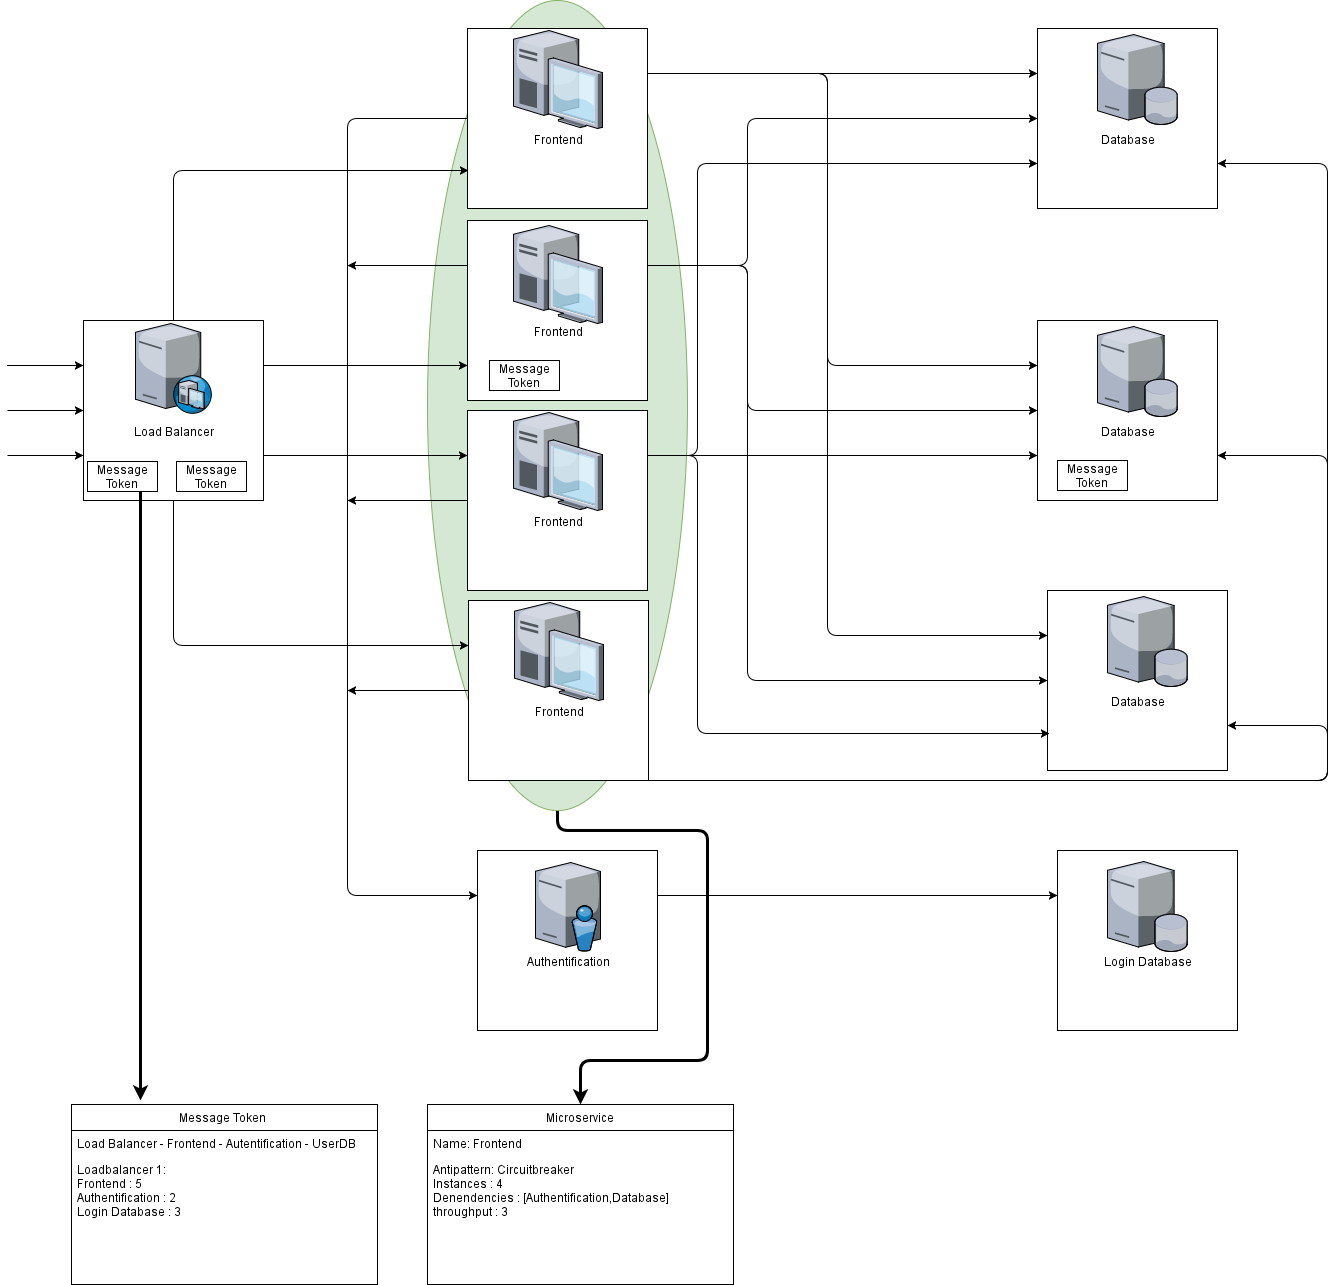
\includegraphics[width=1\textwidth]{figures/MicroserviceSimulatorPicture.png}
		\caption{Simulator System Visualization}
		\label{fig:SystemVisualization}
\end{figure}

\newpage
\begin{figure}
		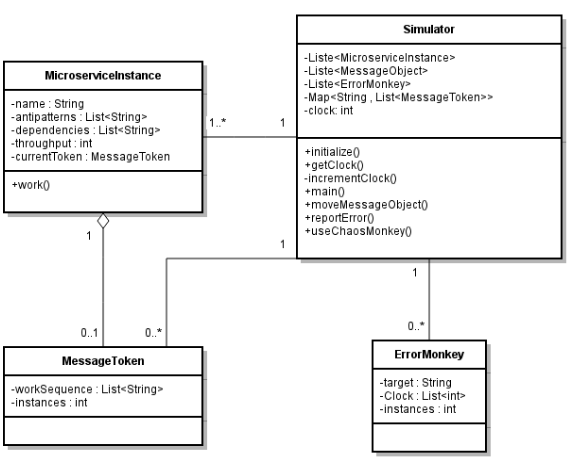
\includegraphics[width=1\textwidth]{figures/Simulator_UML.png}
		\caption{Specified UML Class Diagram}
		\label{fig:SystemUML}
\end{figure}





\section{Simulator internal workflow}
\subsection{MainModelClass}
\subsubsection{Main Method}
The simulator starts by reading all values from the JSON file. Afterwards it proceeds by inserting all metadata into the DesmoJ experiment ( Duration, Seed, Name , ...). Is this done then we continue to start the experiment. DesmoJ is internally calling the init method in which the workflow continues.
\subsubsection{init Method}
Now that the init method was called the simulator creates all data structures belonging to the a micro service(Idle queue, Task queue, ..).To identify a specific micro service the simulator assigns an internal id to each. After creating the general data structures each instance of a micro service is created. Instances also get their values assigned (Resources) and are also mapped to the internal micro service id. 
\subsubsection{doInitialSchedules Method}
Now that the dependence system with all according values is created in DesmoJ the actual experiment can start. Because the simulator uses an event based model this method is called by DesmoJ to start the system and create the initial events. Initial events are called generators in the JSON file. Generators permanently generate new input requests in the specific micro service. Chaos monkeys are also initial events that delete the number of instances specified in JSON file. Is an event generated and the scheduled time meets the actual time in simulation the event gets started and the "workflow" continuous in StartMicroserviceEvent.
\subsection{StartMicroserviceEvent}
Is a micro service event started the message object get placed in the idle queue for the relevant micro service. Is there still open capacity for the responsible micro service the message object gets removed from the idle queue and "work" can start. To know which operations of the micro service are executed a random seed based value is calculated and compared to the probability that the operation is executed. The same applies to dependencies that the service might have. To start "work" on the current task CPU gets removed from the maximal available CPU and a micro service stop event gets scheduled based on the time that a task needs to be finished in this specific micro service. The time between a start event is executed and a stop event is called is the time in which work is supposed to be done. Since this is a simulator the work is not actually done but a thread  and CPU are occupied for this time. 
\subsection{StopMicroserviceEvent}
A StopMicroserviceEvent is called after work has been done in a micro service. CPU gets freed for the micro service instance, the thread in which the current work task was done does no longer exist and the next operations get scheduled for the next available time period(instantly after the finishing of the current task: right now). 


\subsection{Entities}
The name already says it but for clarification all classes located in entities are only holding data and don't contain program logic. Message objects that are a entity represent "work". Message objects know the way they where traversing through the simulated system and therefore can be passed backwards after all operations are done on which they where used.

\section{Input - The JSON File}

This section explains how an correct input file works. For this purpose one micro service of a micro service architecture  is shown in figure \ref{fig:FinalInputMicroServices} and explained. In figure \ref{fig:FinalInputSystemInformation} it is explained how other meta experiment information such as chaos monkeys or system simulation time are inserted into the simulator.

\subsection{System Meta Data Input}
All line references in this subsection reference figure \ref{fig:FinalInputSystemInformation}.

\subsubsection{Simulation}
The key "simulation" (line 2) requires an JSON object that has five values.
\begin{itemize}
\item "experiment" (line 4) name of the experiment no actual importance to the simulator. A String is required. 
\item "model"  (line 5) name of the model no actual importance to the simulator. A String is required.
\item "duration" (line 6) requires an Integer. This integer states how many time units the experiment is going to run. 
\item "datapoints" (line 7) requires an Integer. The Integer states how many data points are taken during the experiment. This value is important since it represents the data points that are later on shown in the graphs to evaluate the experiment results
\item "seed" (line 8) requires an Integer. The seed is there to be a base on random values. Experiments wiht the same input and the same seed will always result the same output. 
\end{itemize}

\subsubsection{Generators}
The key "generators" (line 20) requires an array of objects. Each object is an entry point towards the system since all micro services and dependencies point towards an existing micro service. The entry point is usually just a head node (load balancer) but the simulator allows any number of generators. 
\begin{itemize}
\item
"time" (line 23) requires an Integer. The values states the interval of time units in which new requests are beeing generated
\item
"microservice" (line 24) requires a String. The String is the "name" value of a micro service on which the entry point from the outside points.
\item
"operation" (lien 25) is the operation that is called in the referenced micro service.  
\end{itemize} 

\subsubsection{Chaos Monkeys}
"chaosmonkeys" is an array that requires object with three values.
\begin{itemize}
\item 
"time" requires an Integer. The values means that to the given time period the monkey starts to act.
\item 
"microservice" requires a String that is the name of a micro service in this existing architecture.
\item 
"instances" requires an Integer. The value means that the stated number is deleted at the given time unit. 
\end{itemize}


\subsection{Micro Service Input}
All line references in this subsection reference figure \ref{fig:FinalInputMicroServices}.
\subsubsection{Micro Service}

All micro services are written into an array. The key value for this array is called "microservices" (Line 2-3). 
Each micro service contains four fields. 
\begin{itemize}
\item
The field "name" (line 5) states the name of the current micro service as a String. The name of a micro service is relevant because it is used as a reference in dependencies for operation targets. 
\item
The field "instances" (line 6) displays how many instances of a the current micro service are simulated. The here required value is an Integer.
\item 
"CPU" requires one Integer. (line 7) The inserted value states how many mega hertz (Mhz) a single instance of this current micro service has to distribute to its own operations.  
\item 
"operations" (line 8) is the key value for an array of operations that this micro service has to possibly work on. Each object in this array contains multiple values that are explained in the following subsection. 
\end{itemize}


\subsubsection{Operations}  
\begin{itemize}
\item "name" (line 11) field requires a String value as name of the current operation. The name of a operation is important because it is used as a reference in dependencies for operation targets.
\item 
"pattern" (line 12) requires a String to state the resilience pattern that the current micro service uses. (MAY CHANGE IN THE FUTURE) 
\item "duration" (line 13) requires an Integer value that states how long this operation needs to run from start to finish. The time unit used is seconds and can not be changed. The minimum time unit is one second. 
\item 
"CPU" (line 14) states how much CPU this operation requires. Like the value in micro service this requires an Integer and is represented in mega hertz (Mhz). 
\item "depencencies" (line 15) is the key value for an array. This array contains operations (in other or the same micro service) that are executed after the current operation is finished. The array can be left empty if there are no following calls after an operation is finished. Each dependency is an object containing three values that are explained in the following subsection.
\end{itemize}

\subsubsection{Dependencies} 
\begin{itemize}
\item
"operation" (line 18) requires a String. It is the name of the operation which is going to be executed.
\item 
"service" (line 19) requires the name of an specified micro service. The String points towards an micro service that contains the operation named above. 
\item "probability" (line 20) requires an Double value that between 0.0 and 1.0. The Double value states a percentage chance on which the named operation is called. The probability is rolled against an random value based on the "seed" given for this experiment. This means that the experiment is deterministic for the same set of values and seed.  
\end{itemize} 


\subsection{Exmaple} The operation "register" in micro service "Gateway" is called. For the next 4 time units a single thread of one instance of the micro service Gateway works on an "register" operation. This operation takes 300 Mhz of available CPU form the current instance. After the operation has finished the seed roles a value between 0 and 1 end evaluates whether the dependent operation "save" in micro service "Authentication" is going to be started. 
\end{itemize}




\begin{figure}
\begin{lstlisting}[style=JSON]
{
  "simulation":
  {
    "experiment" : "Desmoj_Microservice_Experiment",
    "model" : "Simple microservice model",
    "duration" : 50,
    "datapoints" : 50,
    "seed" : 2298
  },
  "microservices" :
  [ 
.......
.......
.......
.......
.......
.......
.......
  ],
 "generators" :
   [
     {
       "time" : 1,
       "microservice" : "Gateway",
       "operation" : "update"
     },
     {
       "time" : 50,
       "microservice" : "Backup",
       "operation" : "register"
     }
   ],
   "chaosmonkeys" :
   [
     {
       "time" : 1000,
       "microservice" : "Database",
       "instances" : 1
     },
     {
       "time" : 1000,
       "microservice" : "Gateway",
       "instances" : 1
     }
   ]
}\end{lstlisting}
	\caption{Final Input Structure: Meta Information about the System }
	\label{fig:FinalInputSystemInformation}
\end{figure}

\begin{figure}
\begin{lstlisting}[style=JSON]

  "microservices" :
  [
    {
      "name" : "Gateway",
      "instances" : 10,
      "CPU" : 3500,
      "operations" :
      [
        {
          "name" : "register",
          "pattern" : "Circuit Breaker",
          "duration" : 4,
          "CPU" : 300,
          "dependencies" :
          [
            {
              "name" : "save",
              "service" : "Authentication",
              "probability" : 0.7
            }
          ]
        },
        {
          "name" : "update",
          "pattern" : "Circuit Breaker",
          "duration" : 1,
          "CPU" : 800,
          "dependencies" : 
          [
            {
              "name" : "save",
              "service" : "Order",
              "probability" : 0.8
            }
          ]
        }
      ]
    },
    {
      "name" : "Authentication",
      "instances" : 5,
      "CPU" : 3500,
      "operations" : ......
}\end{lstlisting}
	\caption{Final Input structure: The above JSON is the final input structure which represents the microservice architecture in the simulation.}
	\label{fig:FinalInputMicroServices}
\end{figure}


\begin{center}
--------------------------------------\newline

	TODOLISTE
 
	\paragraph{Execution}
	Validate input\newline
	Failure\newline
	 
	Types of failures:\newline
	Failure of one service\newline
	Failure of multiple services\newline
	 
	Failure modes:\newline
	Static \newline
	Dynamic \newline
	Event driven/Triggered \newline
	 
	Types of reliability patterns: \newline
	Circuit breaker \newline
	Client-side load balancing \newline
	 
	\paragraph{Metrics} 
	How does the failure propagate \newline
	Did the fail-safe measures (circuit breaker, etc.) work \newline
	Systemrun was successful \newline
	 
	 
	TODO - RESEARCH:
	Occurring failure types 
	Reliability patterns
	Metrics
	--------------------------------------\newline
\end{center}

	\newpage

\section{Simulatordocumentation}\label{sec:documentation}
\begin{itemize}
\item struktur des programms
\item probleme in der implementierung 
\item 

\end{itemize}

\section{Conclusions}\label{sec:conclusions}

  These are my conclusions.

\bibliography{template}

\end{document}
